%27May2021 version. 
\documentclass[reqno]{amsart}
\usepackage{amsmath, amssymb, latexsym, amsthm, amsfonts, mathrsfs,
  amscd,color, bbm, tikz, tikz-cd}
\usepackage{scalerel,stackengine, setspace}
\stackMath
\newcommand\reallywidehat[1]{%
\savestack{\tmpbox}{\stretchto{%
  \scaleto{%
    \scalerel*[\widthof{\ensuremath{#1}}]{\kern-.6pt\bigwedge\kern-.6pt}%
    {\rule[-\textheight/2]{1ex}{\textheight}}%WIDTH-LIMITED BIG WEDGE
  }{\textheight}% 
}{0.5ex}}%
\stackon[1pt]{#1}{\tmpbox}%
}
\parskip 1ex
\doublespacing

%\newcommand{\diff}{\textnormal{ d}}


%\usepackage{prelim2e}   %preliminary version
%\usepackage[notref,notcite]{showkeys}  % produces labels on the margin
\renewcommand{\eqref}[1]{(\ref{#1})}   
%for some reason eqref is not supported properly
%\usepackage{showtags}  % produces labels on the margin



%\textwidth=13.5cm


%\textheight=23cm


%\parindent=16pt


%\oddsidemargin=0cm
%
%
%\evensidemargin=0cm



\setlength{\parskip}{0.3cm}
\renewcommand{\baselinestretch}{1.2}
\numberwithin{equation}{section}
\def\q{\quad}
\def\x{\textbf}
\def\mf{\mathbf}
\def\mc{\mathcal}

%%%%%%%%%%%%%%%%%%%%
\theoremstyle{plain}
\newtheorem{theorem}{Theorem}[section]
\newtheorem{lemma}[theorem]{Lemma}
\newtheorem{corollary}[theorem]{Corollary}
\newtheorem{proposition}[theorem]{Proposition}
\newtheorem{conjecture}[theorem]{Conjecture}

\theoremstyle{definition}
\newtheorem{definition}[theorem]{Definition}
\newtheorem{remark}[theorem]{Remark}
\newtheorem{question}[theorem]{Question}
\newtheorem{notation}[theorem]{Notation}
\newtheorem{example}[theorem]{Example}
\newtheorem{claim}[theorem]{Claim}
\newtheorem{ass}[theorem]{Assumption}

\theoremstyle{definition}
\newtheorem{acknowledgement}[theorem]{Acknowledgement}
%%%%%%%%%%%%%%%%%%%%%%%%%%%%%%%%%%%%%%%%%%%

\newcommand{\Q}{{\mathbbm Q}}
\newcommand{\R}{{\mathbbm R}}
\newcommand{\Z}{{\mathbbm Z}}
\newcommand{\C}{{\mathbbm C}}
\newcommand{\N}{{\mathbbm N}}
\newcommand{\F}{{\mathbbm F}}
\newcommand{\A}{{\mathbbm A}}
%\newcommand{\P}{{\mathbf P}}
%\newcommand{\1}{{\mathbbm 1}}

\newcommand{\lb}{\left(}
\newcommand{\rb}{\right)}
\newcommand{\noi}{\noindent}
\newcommand{\ve}{\varepsilon}
\newcommand{\la}{{\langle}}
\newcommand{\ra}{{\rangle}}
\newcommand{\ife}{{\delta_{\Omega}}}
\newcommand{\modp}{(\textnormal{mod }p)}
\newcommand{\modq}{(\textnormal{mod }q)}
\newcommand{\ep}{\varepsilon}
\newcommand{\da}{f_{\delta_{{\mathbbm{A}}^1}}}
\newcommand{\tr}{\textnormal{Tr}}
\newcommand{\deter}{\textnormal{Det}}

\begin{document}



\title[Short running title]{ Same as Title of the article}
%\date{\today}

\author{Authors name}

\address{Author address}  
\email{Author email}

%\subjclass[2010]{Primary 11T24, Secondary 20C33}


%\maketitle

\begin{titlepage}
   \begin{center}
        
       \Huge     
       \textbf{\color{blue} Title of the Article}
       
       \vspace{0.5cm}
       \LARGE
       \textit{A survey article written in fulfillment of}

        \vspace{0.5cm}
       \LARGE
       \textbf{Apprenticeship program,}


        \huge
        \textbf{Lodha Genius Programme}

        
       \vspace{1.5cm}
       \Large
        by
            
       %\vspace{0.2cm}
        \huge
       \textbf{\color{blue} Name of the Author}
       
        \LARGE
        \textit{\color{blue} affiliation of the author}
        
       \vspace{1.5cm}

       \Large
       under the supervision of
       
       %\vspace{0.3cm}
       \huge
       \textbf{Dr. Niladri Patra}

       \LARGE
       \textit{Ashoka University,\\ 
       Plot No. 2, Rajiv Gandhi Education City,\\
       National Capital Region, P.O. Rai,\\
       Sonepat, Haryana-131029, India}
       
            
   \end{center}
\end{titlepage}

\begin{abstract}
    Here you will write the abstract of the article. No references to inside the article or bibliography is allowed here. Any mathematical notation that is not universally well-defined can not be used here without its definition. For example, $\N, \R, \C$ are universally known to denote the set of natural numbers, set of real numbers, and set of complex numbers, respectively, while any notation used for Legendre symbol or multiplier of a fixed point or a congruence residue class are not universally known.  
\end{abstract}

\maketitle


\section{Introduction}

 
\section{Prerequisite}

    \subsection{Subsection 1} An example of citing an article from bibliography, here is \cite{calling_card_1}.

    \subsection{Subsection 2}

\section{Notations}
\begin{lemma}\label{schwartz_lemma}
    Schwartz Lemma
\end{lemma}

\section{Attracting Fixed points}
    \begin{definition}
        Given a map $f$ and a fixed point $p$, we call the point \textit{topologically attracting}, if there exists a neighborhood $U$ of $p$, such that the family of functions $\{f^{\circ n}\}_{n \in \mathbb{N}}$ converges uniformly to the constant function $g(z) = p$ on U.
    \end{definition}
    \begin{figure}
        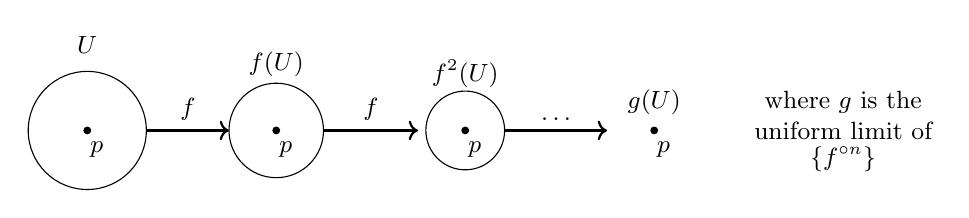
\begin{tikzpicture}[every node/.style={font=\small}, scale=1.2]
            
            % Original neighborhood and point
            \node[circle, draw, minimum size=1.5cm] (U) at (0,0) {};
            \node[fill=black, circle, inner sep=1pt] at (0,0) {};
            \node at (0.1,-0.2) {\( p \)};
            \node at (0,0.9) {\( U \)};
            \draw[->, thick] (U) -- ++(1.5,0) node[midway, above] {\( f \)};
            
            % First image under f
            \node[circle, draw, minimum size=1.2cm] (fU) at (2,0) {};
            \node[fill=black, circle, inner sep=1pt] at (2,0) {};
            \node at (2.1,-0.2) {\( p \)};
            \node at (2,0.7) {\( f(U) \)};
            \draw[->, thick] (fU) -- ++(1.5,0) node[midway, above] {\( f \)};
            
            % Second image under f
            \node[circle, draw, minimum size=1cm] (f2U) at (4,0) {};
            \node[fill=black, circle, inner sep=1pt] at (4,0) {};
            \node at (4.1,-0.2) {\( p \)};
            \node at (4,0.6) {\( f^2(U) \)};
            \draw[->, thick] (f2U) -- ++(1.5,0) node[midway, above] {\( \dots \)};
            
            \node[fill=black, circle, inner sep=1pt] at (6,0) {};
            \node at (6.1,-0.2) {\( p \)};
            \node at (6,0.3) {\( g(U) \)};
            
            \node at (8,0.3) { where $g$ is the};
            \node at (8,0) { uniform limit of};
            \node at (8,-0.3) { $\{f^{\circ n}\}$};
        \end{tikzpicture}
    \end{figure}
    One can think of this as a point, which has a neighborhood which is shrunk down further and further under repeated action by $f$. After infinite iterations of $f$, this neighborhood will be shrunk down to just the point. To characterize this, we use the multiplier.
    \begin{lemma}
        A fixed point $p$ for a holomorphic function $f$ is topologically attracting if and only if its multiplier $\lambda$ satisfies $|\lambda | < 1$
    \end{lemma}
    \begin{proof}
        \begin{samepage}
        $(|\lambda| < 1 \implies topologically \ attracting)$\\
        First, recall that through m\"obius conjugations, we can send $p$ to $0$, argue there, and apply the inverse transformation to bring the arguments back to $p$. We aim to find a neighborhood that $f$ contracts geometrically. using that, we can show that the family of iterates of $f$ will converge geometrically to the constant $0$ function. So, we show that $\exists r$ such that $\forall z \in \mathbb{D}_r$ 
        \[
            f(z) \leq c \cdot |z|
        \]
        where $c < 1$. Choose any $c$ such that $|\lambda| < c < 1$. 

        WLOG, let $f(0) = 0$. Taylors thorem tells us that for some small enough $r_0$, $ f(z) = \lambda z + O(z^2)$ on $\mathbb{D}_{r_0}$. That is,
        \begin{align}
        &|f(z) - \lambda z | \leq  c_0\cdot |z^2| & \forall z \in \mathbb{D}_{r_0} \notag\\
        &|f(z)| \leq |\lambda z| + c_0 \cdot |z^2| = (|\lambda| + c_0|z|)\cdot |z| \label{4.1}
        \end{align}
        Since this holds on $\mathbb{D}_{r_0}$, it also holds on $\mathbb{D}_{r}$ for all $r \leq r_0$. By the archimedian principle, we know that there exists a small enough $r_1$ such that $0 < c_0\cdot r < c - |\lambda| \implies |\lambda| + c_0\cdot r < c$. Setting $r = \min \{r_0, r_1\}$ and continuing from \eqref{4.1} we can say that, 
        \[
        |f(z)| \leq (|\lambda| + c_0\cdot r)\cdot |z| < c \cdot |z| \hspace{2cm} \forall z \in \mathbb{D}_r 
        \]
        Now, the claim is that on this neighborhood $\mathbb{D}_r$ of 0, the family of functions $\{f^{\circ n}\}$ converges uniformly. So, $\forall z \in \mathbb{D}_r$,
        \[
        \ |f(z)| < c \cdot |z| < c \cdot r
        \]
        since $c<1$, $f(z)$ is in $\mathbb{D}_r$. So we can also say $\forall z \in \mathbb{D}_r$
        \[
         \ |f \circ f(z)| < c \cdot |f(z)| < c^2 \cdot r 
        \]
        Continuing this argument,
        \[
         |f^{\circ n}(z)| < c^n |z| < c^n r
        \]
        This converges uniformly to $0$ as $n \to \infty$. So $0$ is topologically attracting.\\
        \end{samepage}

        $(topologically \ attracting \implies |\lambda| < 1)$
        If $0$ is a topologically attracting fixed point, then there exists a neighborhood $U$ of $0$ such that $\{f^{\circ n}\}$ converges uniformly to the constant $0$ function on $U$. So, for all $\epsilon >0$ there exists an $N > 0$ such that $\forall n > N$,
        \[
            |f^{\circ n}(z)| < \epsilon \quad \quad \forall z \in U
        \]
        Consider the disk $\mathbb{D}_{\epsilon} \subset U$. The above statement implies that $\mathbb{D}_{\epsilon}$ is mapped onto a proper subset of itself by some iterate $f^{\circ n}$. Using Schwartz lemma (\ref{schwartz_lemma}) on this iterate and $\mathbb{D}_{\epsilon}$, we get that the multiplier of $f^{\circ n}$, which is $\lambda^n$ satisfies $|\lambda^n| < 1$. But this implies that $|\lambda|<1$.

    \end{proof}
    \begin{theorem}{Koenigs Linearisation theorem} \\
        Given a geometrically attracting fixed point or a repelling fixed point of $f$, there exists a local holomorphic change of co-ordinates $\phi$, such that $\phi \circ f \circ \phi^{-1}(w) = \lambda w$ for all $w$ in some neighborhood of 0. Further, $\phi$ is unique upto multiplication by a constant.
    \end{theorem}
    A restatement of the above, is that the following diagram commutes
    \[ 
    \begin{tikzcd}
        U \arrow{r}{f} \arrow[swap]{d}{\phi} & f(U) \arrow{d}{\phi} \\%
        \mathbb{D}_\epsilon \arrow{r}{w \mapsto \lambda w} & \mathbb{D}_\epsilon
    \end{tikzcd}
    \]
    \begin{proof}
        \textbf{Existence:} First we show that such a function exists. Define the following family of functions, $\{\phi_n\}$ as
        \[
            \phi_n(z) = \frac{f^{\circ n}(z)}{\lambda^n}  
        \]
    \end{proof}
    \subsection{Subsection 1}

    
    
    \subsection{Subsection 2} 

\section{Main Section 2}\label{main2}

    \subsection{Subsection 1}\label{sub1}
     You can also label and summon sections and subsections as in Section \ref{main2}, Subsection \ref{sub1}.
    
    \subsection{Subsection 2} 

\section{Applications and connections}

    \subsection{Subsection 1}
    
    \subsection{Subsection 2} 

\section*{Acknowledgement}
    Here you can write your acknowledgement.

    First Line, Thank me, hehe.

    Second Line, Thank LGP programme.

    Third Line onwards, Thank whoever you want.


\begin{thebibliography}{10}
    \bibitem[1]{calling_card_1}
        Arfeux, Matthieu \& Jan Kiwi.  Irreducibility of periodic curves in cubic polynomial moduli space. (2020), Proceedings of London Mathematical Society, to appear. https://api.semanticscholar.org/CorpusID:229923967
    \bibitem[2]{calling card 2}
        Blanchard, Paul, Robert L. Devaney \& Linda Keen.  The dynamics of complex polynomials and automorphisms of the shift. Inventiones mathematicae 104 (1991): 545-580. https://doi.org/10.1007/BF01245090
    \bibitem[3]{calling card 3}
        Buff, Xavier, Adam L. Epstein \& Sarah Koch.  Prefixed curves in moduli space. American Journal of Mathematics 144, no. 6 (2022): 1485-1509. doi:10.1353/ajm.2022.0036.
    \bibitem[4]{calling card 4}
        Benedetto, Robert L. \& Vefa Goksel.  Misiurewicz polynomials and dynamical units, part I. International Journal of Number Theory: Vol. 19, No. 06, pp. 1249-1267 (2023). https://doi.org/10.1142/S1793042123500616
    \bibitem[5]{calling card 5}
        Benedetto, Robert L. \& Vefa Goksel. Misiurewicz polynomials and dynamical units, Part II. (2022) ArXiv. https://doi.org/10.48550/arXiv.2203.14431
    
   
\end{thebibliography}

\end{document}
